\documentclass[preprint,12pt]{elsarticle}

\usepackage{amsmath,amssymb,amsthm}
\usepackage{graphicx}
\usepackage{booktabs}
\usepackage{makecell}
\usepackage{rotating}
\usepackage[hidelinks]{hyperref}
\usepackage{lineno}
\usepackage{xcolor}
\usepackage{microtype}
\usepackage[section]{placeins}
\setlength{\emergencystretch}{2em}

\newtheorem{proposition}{Proposition}
\newtheorem{theorem}{Theorem}
\newcommand{\appref}[1]{\ref{#1}}
\makeatletter
\newcommand{\inputtable}[1]{\@@input #1 }
\makeatother
\journal{Sustainable Operations and Computers}

\begin{document}

\begin{frontmatter}

\title{Anticipating demand in carbon-aware scheduling across data centres: guarantees and fair carbon attribution}

\author{Quang-Vinh Dang\corref{cor1}}
\ead{vinh.dq4@buv.edu.vn}
\cortext[cor1]{Corresponding author. ORCID: 0000-0002-3877-8024}
\affiliation{organization={British University Vietnam},
            city={Hung Yen},
            country={Vietnam}}

\begin{abstract}
Shifting deferrable jobs to cleaner times and places cuts data-centre emissions, but online schedulers act before future grid conditions and jobs are known. We formulate multi-site, deadline-constrained scheduling of bag-of-tasks jobs as a minimum-cost flow problem and study CARMA (Carbon-aware Anticipatory Receding-horizon Multi-site Allocation), which adds ``ghost jobs'' for expected arrivals to each hourly plan. Uncertainty about demand alone forces any online algorithm, even with perfect carbon forecasts, to a competitive ratio of $\Omega(\sqrt{\theta})$, where $\theta$ is the ratio of highest to lowest unit emission cost. Under explicit assumptions (a backstop resource, episodes within the planning window), CARMA never misses a deadline and is optimal under exact predictions; these assumptions do not hold in the weekly experiments. On 2024 regional grid data for Great Britain, CARMA comes within 8.0--9.8\% of the clairvoyant optimum, against 15.5--16.3\% for the best baseline without demand information. On four further fleets covering Europe, North and South America and Oceania, its gap is 2.7--5.8\% against 4.4--13.0\%. A scenario-based stochastic lookahead with the same demand information is level with CARMA or at most 1 point better, but needs 12--37 times more computing time. A trace-derived workload with a biased demand profile gives 21.2\% against 27.5\%. Under a stylised marginal-emission proxy, however, achievable reductions shrink to 14\% and CARMA's edge becomes small. Dual prices of the pooled problem give a carbon attribution in the core of the hindsight pooling game, whereas origin- and host-based accounting violate coalitional stability in every week.
\end{abstract}

\begin{keyword}
Carbon-aware computing \sep Data centre scheduling \sep Competitive analysis \sep Minimum-cost flow \sep Cooperative cost allocation \sep Carbon intensity forecasting
\end{keyword}

\end{frontmatter}

\linenumbers

\section{Introduction}\label{sec:intro}

Data centres are among the fastest-growing electricity consumers. Efficiency gains kept their energy use nearly flat through the 2010s even as computing output grew several-fold~\cite{masanet2020recalibrating,shehabi2016united}. That buffer is now thinning, and information and communication technology accounts for an estimated 2.1--3.9\% of global greenhouse-gas emissions~\cite{freitag2021real}. Large machine-learning workloads have drawn particular attention~\cite{strubell2019energy,patterson2022carbon,dodge2022measuring}. The carbon intensity of grid electricity varies by a factor of ten or more across regions and hours, driven by the output of wind, solar and dispatchable plant~\cite{staffell2017measuring}. Operators can therefore cut emissions without new hardware by moving flexible work to cleaner places and times. Such \emph{carbon-aware computing}~\cite{radovanovic2023carbon,bashir2021enabling} is an operations problem: capacity is finite, deadlines bind, and both the grid and the job stream are uncertain.

Batch jobs such as model training, analytics, rendering and backups are a natural target, because they tolerate some delay. Previous work has shown the potential of temporal shifting (running later)~\cite{wiesner2021lets,goiri2012greenhadoop,hanafy2023carbonscaler} and of spatial shifting (running elsewhere)~\cite{liu2011greening,zheng2020mitigating}. It has also shown their limits. Sukprasert et al.~\cite{sukprasert2024limitations} found that practical reductions from spatio-temporal shifting fall well short of idealised bounds. Most methods are evaluated with a scheduler that reacts to the jobs it has already seen, using point forecasts of carbon intensity. Two questions have received less attention. First, how much is lost because an online scheduler does not know which jobs will arrive next? Second, does it pay to price the uncertainty of carbon-intensity forecasts into scheduling decisions?

This paper answers both questions with a new algorithm and a forecasting model, evaluated on three years of real regional grid data for Great Britain. It makes four contributions.
\begin{enumerate}
\item \textbf{Formulation.} We state multi-site, deadline-constrained, width-limited scheduling of deferrable bag-of-tasks jobs, including the emissions of data transfer, as a minimum-cost flow problem (Proposition~\ref{prop:flow}). Offline clairvoyant optima and every online planning step can therefore be computed exactly and quickly by network simplex. We also prove that myopic receding-horizon scheduling can be arbitrarily worse than the clairvoyant optimum even with perfect carbon forecasts (Proposition~\ref{prop:myopic}).
\item \textbf{Algorithm.} We propose CARMA (Carbon-aware Anticipatory Receding-horizon Multi-site Allocation). At every hour, CARMA adds \emph{ghost jobs} to its planning network. These represent expected arrivals, learned from the operator's history, so the planner reserves scarce low-carbon capacity for work that has not yet arrived. The planning problem stays a single min-cost flow and decisions take tens of milliseconds.
\item \textbf{Forecasting model.} We develop a probabilistic 1--24-hour carbon-intensity forecaster. It consists of direct gradient-boosted models with horizon-wise normalised conformal calibration and adaptive conformal inference, which holds coverage under the strong decarbonisation drift seen in 2024. Its calibrated quantiles let us test risk-adjusted carbon pricing inside the scheduler.
\item \textbf{Evidence.} Across 52 out-of-sample weeks, three load levels and two operating regimes, we compare CARMA with five implementable online baselines, clairvoyant and ablated variants, and the clairvoyant oracle. The results separate the value of anticipating demand from the value of better carbon forecasts, and show when each matters.
\end{enumerate}

The results carry an operational message. Once spatial shifting is allowed, the dominant loss comes from demand myopia, not from forecast error. Anticipating demand cuts the gap to the clairvoyant optimum by a factor of 2.2--3.0. By contrast, perfect carbon foresight or risk-averse carbon pricing adds little once demand is anticipated. Without migration, temporal shifting alone achieves much smaller reductions. The forecast-driven planners are then within 4--6\% of the optimum, and the remaining gap is due almost entirely to forecast error. The rest of the paper is organised as follows. Section~\ref{sec:related} reviews related work. Section~\ref{sec:methods} presents the model, the forecaster, CARMA and the experimental design. Section~\ref{sec:results} reports results, Section~\ref{sec:discussion} discusses implications and limitations, and Section~\ref{sec:conclusion} concludes.

\section{Related work}\label{sec:related}

\paragraph{Carbon-aware workload shifting} Early green data-centre schedulers matched deferrable jobs to on-site solar production, for example GreenSlot~\cite{goiri2011greenslot} and GreenHadoop~\cite{goiri2012greenhadoop}. Other work exploited electricity-price and carbon differences across sites through geographical load balancing~\cite{rao2010minimizing,liu2011greening} and dynamic right-sizing~\cite{lin2013dynamic}. With public carbon-intensity feeds, attention moved to grid emissions. Wiesner et al.~\cite{wiesner2021lets} quantified the reductions from temporal shifting in several regions, including Great Britain, and proposed forecast-based lowest-window scheduling. Google's carbon-intelligent compute system sets next-day virtual capacity curves from carbon and demand forecasts~\cite{radovanovic2023carbon}. CarbonScaler varies the allocation of elastic jobs with carbon intensity~\cite{hanafy2023carbonscaler}. Ecovisor exposes the energy system to applications~\cite{souza2023ecovisor}. Carbon Explorer weighs scheduling against investment in renewables and storage~\cite{acun2023carbon}. Load migration between data centres can absorb curtailed renewable generation~\cite{zheng2020mitigating}, and data-centre demand response has been surveyed in~\cite{wierman2014opportunities}. Sukprasert et al.~\cite{sukprasert2024limitations} bound the potential of spatio-temporal shifting across 123 regions and find that simple policies capture most of the achievable benefit. Our study complements theirs by identifying \emph{which} information limits online schedulers when capacity at clean sites is scarce.

\paragraph{Energy-aware scheduling in operations} Energy-efficient scheduling is a mature topic in manufacturing operations~\cite{gahm2016energy}, and green scheduling models have appeared in this journal, for example for parallel machines with job splitting~\cite{asadpour2022green} and for cloud resource allocation~\cite{sharma2024efficient}. Most such models are deterministic and solved offline, often with metaheuristics. We instead exploit exact network-flow structure~\cite{ahuja1993network,orlin1997polynomial} and embed it in an online lookahead policy. In the taxonomy of Powell~\cite{powell2019unified}, CARMA is a deterministic lookahead policy with a modified (anticipatory) model, in the spirit of model predictive control~\cite{rawlings2017model,mayne2000constrained}.

\paragraph{Carbon-intensity forecasting} Forecasts of grid carbon intensity use statistical decomposition~\cite{bokde2021short}, machine learning with many exogenous drivers~\cite{leerbeck2020short}, day-ahead regression for building demand response~\cite{lowry2018day}, and hierarchical models of the generation mix, as in CarbonCast~\cite{maji2022carboncast}. For Great Britain, NESO publishes regional forecasts through its Carbon Intensity API~\cite{nesoapi}. These studies focus on point accuracy. For decisions, calibrated uncertainty matters as well. Conformal prediction~\cite{vovk2005algorithmic,lei2018distribution,angelopoulos2023conformal} provides distribution-free intervals and has been extended to quantile regression~\cite{romano2019conformalized}, to multi-horizon~\cite{stankeviciute2021conformal} and dynamic time series~\cite{xu2023conformal}, and to arbitrary distribution shift through adaptive conformal inference~\cite{gibbs2021adaptive}. We use these tools to build a calibrated forecaster and to test, in a controlled way, whether risk-adjusted carbon costs improve scheduling. The question is motivated by the optimizer's curse~\cite{smith2006optimizer} and by the robust-optimisation view that point-estimate solutions can be fragile~\cite{bental2000robust,bertsimas2004price}.

\section{Material and methods}\label{sec:methods}

\subsection{Problem setting}\label{sec:problem}

We consider an operator that runs a set $\mathcal{S}$ of data-centre sites connected by a wide-area network. Time is divided into hourly slots $t=0,1,2,\dots$ Deferrable batch jobs arrive online. Job $j$ is released at the start of hour $a_j$ at origin site $o_j\in\mathcal{S}$. It carries $w_j$ server-hours of work made of independent tasks (a bag of tasks), can use at most $m_j$ servers concurrently, and must finish before the start of hour $d_j>a_j$. Work may be paused and resumed, and any part of it may run at a site other than its origin. Remote execution requires moving input data. At site $s$ and hour $t$, $K_s(t)$ servers are free for batch work once the interactive load has been served.

Let $I_s(t)$ be the average carbon intensity of the electricity supplied to site $s$ during hour $t$ (gCO$_2$/kWh). Executing one server-hour of job $j$ at site $s$ during hour $t$ emits
\begin{equation}\label{eq:unitcost}
c_{o_j s}(t) = e\,\mathrm{PUE}_s\, I_s(t) + \mathbf{1}[s\neq o_j]\,\delta\,\eta\,\tfrac{1}{2}\big(I_{o_j}(t)+I_s(t)\big),
\end{equation}
where $e$ is the IT energy per server-hour, $\mathrm{PUE}_s$ is the power usage effectiveness of site $s$, $\delta$ is the data volume moved per migrated server-hour and $\eta$ is the energy intensity of network transfer (kWh/GB). The transfer term charges network energy at the mean intensity of the two endpoints. With decision variables $x_{js}(t)\ge 0$ (server-hours of job $j$ run at site $s$ in hour $t$), the offline version of the problem is the linear programme
\begin{align}
\min_{x,u\ge 0}\quad & \sum_j\sum_{s}\sum_{t=a_j}^{d_j-1} c_{o_j s}(t)\,x_{js}(t) + \sum_j \Pi\, u_j \label{eq:obj}\\
\text{s.t.}\quad & \textstyle\sum_{s}\sum_{t=a_j}^{d_j-1} x_{js}(t) + u_j = w_j && \forall j, \label{eq:work}\\
& \textstyle\sum_{s} x_{js}(t) \le m_j && \forall j,\ t\in[a_j,d_j), \label{eq:width}\\
& \textstyle\sum_{j:\,a_j\le t<d_j} x_{js}(t) \le K_s(t) && \forall s,t, \label{eq:cap}
\end{align}
where $u_j$ is work left unfinished at the deadline and $\Pi$ is a lateness penalty much larger than any emission cost. When migration is not allowed, $x_{js}(t)=0$ for $s\neq o_j$. With complete knowledge of arrivals and intensities, the optimum of (\ref{eq:obj})--(\ref{eq:cap}) is a lower bound for every online policy, and we use it as the \emph{clairvoyant oracle}. An online scheduler has to fix $x_{\cdot s}(t)$ at the start of hour $t$. At that point it knows the jobs released so far, the current intensities $I_s(t)$ and nothing more than forecasts of $I_s(t+h)$ and of future arrivals.

\begin{proposition}[Network-flow structure]\label{prop:flow}
Problem (\ref{eq:obj})--(\ref{eq:cap}) is a minimum-cost flow problem on a network with a source, one node per job, one node per (job, hour) pair, one node per (hour, site) pair and a sink. Arc capacities are $w_j$ (source$\to j$), $m_j$ ($j\to(j,t)$) and $K_s(t)$ ($(t,s)\to$ sink). The only arcs with a cost are $(j,t)\to(t,s)$, priced at $c_{o_j s}(t)$, and a slack arc $j\to$ sink priced at $\Pi$.
\end{proposition}
\begin{proof}
Conservation at the job node is Eq.~(\ref{eq:work}). The capacity of arc $j\to(j,t)$ is Eq.~(\ref{eq:width}), conservation at $(j,t)$ splits that hour's work across sites, and the capacity of $(t,s)\to$ sink is Eq.~(\ref{eq:cap}). Conversely, every feasible flow defines a feasible $(x,u)$ with the same cost. The constraint matrix of the flow formulation is a node-arc incidence matrix, in which every column has exactly one $+1$ and one $-1$, so it is totally unimodular.
\end{proof}

Proposition~\ref{prop:flow} has a practical consequence. The oracle and every planning problem solved online (Section~\ref{sec:carma}) can be solved exactly by network simplex~\cite{ahuja1993network}, and integral data (work quantised to $0.01$ server-hours) give integral optimal flows. We use the OR-Tools implementation~\cite{ortools}. On the instances studied, network simplex returned the same objective value as a general-purpose LP solver (HiGHS) to within rounding, and it cut the total run time of the online planners by a factor of about six.

\subsection{Probabilistic carbon-intensity forecasting}\label{sec:forecast}

\paragraph{Point model} For each horizon $h=1,\dots,H$ ($H=24$ h) we fit a direct gradient-boosted regression tree model~\cite{friedman2001greedy} that predicts the change $I_s(t+h)-I_s(t)$ from information available at issue time $t$. Direct per-horizon models avoid the error accumulation of recursive strategies~\cite{taieb2012review}. One model per horizon is pooled across sites, with the site as a categorical feature. The features are the current intensity; differences between the current value and lags of 1, 2, 3, 6, 12 and 23 hours; the value observed at the same hour of the target on the previous day and in the previous week; a 24-hour rolling mean and mean absolute change (volatility); the national (GB) intensity; the regional wind, solar and gas shares; and calendar encodings of the target time (hour of day, day of week, annual sine and cosine). Models are fitted with absolute-error loss, so they estimate the conditional median. We use scikit-learn's histogram gradient boosting~\cite{pedregosa2011scikit} with 400 iterations, learning rate 0.05, 31 leaves and at least 50 samples per leaf. The models use only information available when the forecast is issued, and no weather forecasts. This is deliberate: the goal is a forecaster any operator can build from a public intensity feed.

\paragraph{Conformal upper quantiles} A point forecast $\hat I_s(t+h\,|\,t)$ is turned into calibrated upper quantiles by split conformal prediction~\cite{vovk2005algorithmic,lei2018distribution} with normalised scores. On a calibration window disjoint from training, we compute for each site $s$ and horizon $h$
\begin{equation}
r_{s,h}(t) = \frac{I_s(t+h)-\hat I_s(t+h\,|\,t)}{\sigma_s(t)+\epsilon},
\end{equation}
where $\sigma_s(t)$ is the 24-hour mean absolute hourly change observed at issue time and $\epsilon=5$~gCO$_2$/kWh. For a target level $\beta$, the upper forecast is $U^{\beta}_s(t+h\,|\,t)=\hat I_s(t+h\,|\,t)+\hat q_{s,h}(\beta_{s,h}(t))\,(\sigma_s(t)+\epsilon)$, where $\hat q_{s,h}(\cdot)$ is the empirical quantile function of the calibration scores. Grid carbon intensity is not exchangeable over time: 2024 was markedly cleaner than 2022--2023 (Fig.~\ref{fig:data}). We therefore update the working level online by adaptive conformal inference (ACI)~\cite{gibbs2021adaptive}. Once $I_s(t+h)$ is observed,
\begin{equation}\label{eq:aci}
\alpha_{s,h} \leftarrow \alpha_{s,h} + \gamma\big((1-\beta) - \mathbf{1}[I_s(t+h) > U^{\beta}_s(t+h\,|\,t)]\big),\qquad \beta_{s,h}(t)=1-\alpha_{s,h},
\end{equation}
with step size $\gamma=0.005$. By the ACI result of~\cite{gibbs2021adaptive}, the long-run frequency with which realised intensities exceed $U^\beta$ converges to $1-\beta$ for any data sequence, with no distributional assumption. This matters for the scheduler: the level $\beta$ becomes an interpretable risk dial, and it stays valid under drift. With $\beta=0.5$ the procedure also removes level shifts in the point model (a recalibrated median).

\subsection{CARMA: carbon-aware anticipatory receding-horizon multi-site allocation}\label{sec:carma}

A standard receding-horizon (model predictive control, MPC) scheduler~\cite{rawlings2017model} solves, at every hour $t$, the flow problem of Proposition~\ref{prop:flow} restricted to pending jobs and the window $[t,t+H)$. Future intensities are replaced by forecasts, and only the first hour of the plan is executed. Such a planner is \emph{myopic about demand}: it sees only jobs that have already arrived. The next result shows that this can be arbitrarily costly even when carbon intensities are known exactly.

\begin{proposition}[Myopia can be unboundedly costly]\label{prop:myopic}
Even with perfect intensity forecasts, myopic receding-horizon scheduling has no finite competitive ratio with respect to the clairvoyant oracle.
\end{proposition}
\begin{proof}
Take a clean site $A$ with one server and a dirty site $B$ with ample capacity. Let $c_A(0)=\varepsilon$, $c_A(1)=0$ and $c_B(0)=c_B(1)=c$, and ignore transfer costs. A flexible job ($w=1$, $m=1$) arrives at $t=0$ with deadline $d=2$. An urgent job ($w=1$) arrives at $t=1$ with $d=2$. At $t=0$ the myopic planner sees only the flexible job and defers it to $A$ at $t=1$ (cost $0<\varepsilon$). At $t=1$ both jobs must run in the same hour, one of them at $B$, so the total cost is $c$. The oracle runs the flexible job at $t=0$ and the urgent job at $t=1$, both at $A$, for a total of $\varepsilon$. The ratio $c/\varepsilon$ is unbounded as $\varepsilon\to 0$.
\end{proof}

The mechanism in Proposition~\ref{prop:myopic} is common in practice. Low-carbon capacity is scarce, and a myopic planner spends it on flexible work that could have waited or run elsewhere, leaving urgent jobs that arrive later to run on carbon-intensive capacity. CARMA addresses it by anticipating demand inside the same flow problem, and optionally prices forecast risk.

\begin{figure}[t]
\centering
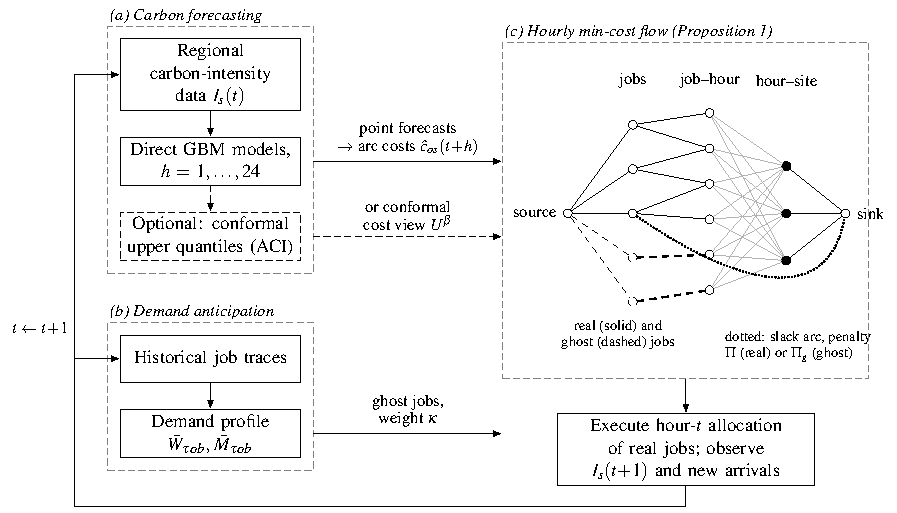
\includegraphics[width=\textwidth]{../figures/fig1_carma.pdf}
\caption{The CARMA decision loop. (a) Probabilistic carbon-intensity forecasts price the job--hour to hour--site arcs. (b) A demand profile learned from past traces generates ghost jobs for expected arrivals. (c) Real jobs (solid) and ghost jobs (dashed) share one min-cost flow network, whose dotted slack arc carries unfinished work to the sink at the lateness penalty. The network is solved exactly every hour, and only the first-hour allocation of real jobs is executed.}
\label{fig:carma}
\end{figure}

\paragraph{Anticipated demand (ghost jobs)} From the operator's own history we estimate, for every hour of the week $\tau$, origin $o$ and window class $b$, the expected work $\bar W_{\tau ob}$ and the expected total width $\bar M_{\tau ob}$ of arriving jobs. Window classes are the bins $\mathcal{B}=\{1,2,4,6,9,13,18,24\}$ hours. A job is assigned to the largest bin not exceeding its window, so ghost jobs are never more flexible than the jobs they represent. At hour $t$, for each $k=1,\dots,\ell$ (the look-ahead), CARMA adds to the planning problem a \emph{ghost job} for every $(o,b)$ with work $\kappa\bar W_{\tau(t+k)ob}$, width $\kappa\bar M_{\tau(t+k)ob}$, release $t+k$ and deadline $\min(t+k+b,\,t+H)$. Ghost jobs compete with real jobs for capacity, but their slack arc is priced at a moderate penalty $\Pi_g$, set to $1.5$ times the largest local unit cost in the window, rather than at $\Pi$. They can therefore reserve clean capacity when it is economical but never force real work to be late. The weight $\kappa\ge 0$ scales how much of the expected demand is anticipated. With $\kappa=0$, CARMA reduces to myopic MPC.

\paragraph{Carbon cost view} Future-hour costs in Eq.~(\ref{eq:unitcost}) are evaluated at a forecast of $I_s(t+h)$; for the current hour ($h=0$) the observed intensity is used. CARMA admits two cost views: the point forecast $\hat I$, or the conformal upper quantile $U^{\beta}$ of Section~\ref{sec:forecast}. The second is motivated by the optimizer's curse~\cite{smith2006optimizer}: selecting the minimum over noisy estimates is biased towards optimism, and a level $\beta>0.5$ penalises uncertain future hours in proportion to their calibrated spread. Whether this risk premium helps is an empirical question, and we treat the cost view as a hyperparameter.

\paragraph{Algorithm} Fig.~\ref{fig:carma} summarises the loop. At each hour $t$, CARMA (i) observes $I_s(t)$, the free capacity and the pending jobs; (ii) builds the cost cube $c_{os}(t+h)$ for $h<H$ from the chosen forecast view; (iii) adds the ghost jobs for hours $t+1,\dots,t+\ell$; (iv) solves the resulting min-cost flow problem exactly; (v) executes the first-hour allocations of the real jobs only; and (vi) after observing the realised intensities, updates the ACI levels by Eq.~(\ref{eq:aci}) when conformal costs are used. Overdue work gets a one-hour window and is served with priority. The planning network has $O\big((n_t+\ell|\mathcal{S}||\mathcal{B}|)\,H\,|\mathcal{S}|\big)$ arcs, where $n_t$ is the number of pending jobs, so each decision takes a few tens of milliseconds (Section~\ref{sec:results}). The hyperparameters $(\kappa,\ell)$ and the cost view are tuned on validation weeks that precede the test period (Section~\ref{sec:tuning}).

\subsection{Baselines}\label{sec:baselines}

We compare CARMA with the following online policies and the oracle. \textbf{ASAP-Local} is carbon-agnostic: it runs work at its origin as soon as possible, earliest deadline first (EDF). \textbf{Greedy-Spatial} also runs work immediately, but at the site that is currently cleanest; this is geographical load balancing without temporal shifting~\cite{liu2011greening}. \textbf{Forecast-Reserve} books, when a job arrives, the cheapest forecast (site, hour) slots in its window that still have capacity, and never revises the booking. This is the lowest-window strategy of~\cite{wiesner2021lets} extended to multiple sites. \textbf{MPC} is the myopic receding-horizon flow scheduler with point forecasts. \textbf{MPC+conformal} uses the conformal upper quantile at the level that was best for MPC on validation data. \textbf{MPC-Perfect} is MPC given the realised intensities, which isolates the value of forecast accuracy. \textbf{CARMA-Perfect} is CARMA given the realised intensities, and \textbf{CARMA+conformal} is CARMA with the best conformal cost view. \textbf{Oracle} solves (\ref{eq:obj})--(\ref{eq:cap}) with full knowledge of arrivals and intensities.

\subsection{Data and experimental design}\label{sec:data}

\paragraph{Carbon intensity} We use half-hourly regional carbon intensity for Great Britain from the Carbon Intensity API of the National Energy System Operator (NESO)~\cite{nesoapi} from 1 January 2022 to 31 December 2024. Values are averaged to hourly resolution. Four regions host the candidate sites: South Scotland, North West England, West Midlands and London. They span the north--south gradient of the British grid, from wind- and nuclear-rich South Scotland to gas-dependent London, and include the main data-centre markets of London, Manchester (North West England) and Birmingham (West Midlands). Gaps (602 of 26{,}304 hours in at least one region) were filled by linear interpolation. The period up to 30 June 2023 is used to train the forecaster, July--September 2023 to calibrate the conformal scores, October--December 2023 to tune the scheduler, and all 52 weeks starting on Mondays in 2024 as the out-of-sample test set.

\paragraph{Sites and energy parameters} Batch capacities are 300, 400, 400 and 600 servers for South Scotland, North West England, West Midlands and London. This reflects a small, clean northern site and a large site in London. Interactive load takes $20\%\pm15\%$ of each site's capacity on a diurnal cycle that peaks in the afternoon. We assume $e=0.4$~kWh per server-hour. The assumed PUE values are 1.15, 1.20, 1.25 and 1.30 from north to south, reflecting free-cooling potential. Migrated work moves $\delta=2$~GB per server-hour at $\eta=0.02$~kWh/GB. This value lies within the wide range of published estimates of transmission energy intensity~\cite{aslan2018electricity}. We vary $\eta$ in a sensitivity analysis.

\paragraph{Workloads} Job arrivals follow a non-homogeneous Poisson process with a diurnal peak in the afternoon and 30\% lower weekend rates. Jobs originate at the four sites with probabilities 0.10, 0.20, 0.25 and 0.45. Width $m_j$ is log-uniform on $[4,64]$ servers and the run time at full width $r_j$ is uniform on $\{1,\dots,6\}$ hours, so $w_j=m_jr_j$. A share $\upsilon$ of jobs is urgent (deadline $=a_j+r_j$, no temporal slack); for the others the window is $\lceil f_j r_j\rceil$ hours with $f_j\sim U[1.5,4]$, capped at 24 hours. The baseline value is $\upsilon=0.3$. The arrival rate is scaled so that the offered load equals a fraction $\rho\in\{0.3,0.5,0.7\}$ of the mean free capacity. Each test episode covers one week of arrivals. We also simulate 24 hours of arrivals before and after the week, so the evaluated week starts and ends under steady-state congestion. Metrics are computed only for jobs released during the week. For each week and load level we draw one workload trace with a fixed seed, and every policy runs on that same trace. The demand profile used by CARMA is estimated from 13 independent historical traces. We study two regimes: \emph{spatio-temporal}, where migration is allowed, and \emph{temporal-only}, where it is not.

\paragraph{Metrics and statistics} The primary metric is operational emissions (tCO$_2$) per week. We report the reduction relative to ASAP-Local and the optimality gap relative to the oracle, the share of work finished late, the share of work executed away from its origin, and the decision time. Policies are compared by paired two-sided Wilcoxon signed-rank tests over the 52 test weeks, with Holm correction across comparisons.

\section{Theoretical guarantees}\label{sec:theory}

This section establishes three kinds of guarantees. The first is a worst-case limit that applies to \emph{every} online scheduler. The second is a set of worst-case and prediction-dependent guarantees for CARMA. The third is a fairness property of the carbon attribution induced by the pooled scheduling problem. Proofs are given in \ref{app:proofs}. Throughout, unit costs (Eq.~(\ref{eq:unitcost}), including any backstop resource introduced below) satisfy $0<L\le c_{os}(t)\le U$, and $\theta=U/L$ denotes the \emph{carbon-intensity ratio}. A positive floor $L$ holds as soon as the embodied emissions of servers, or a non-zero minimum grid intensity, are counted. An online algorithm is \emph{$\rho$-competitive} if its emissions never exceed $\rho$ times those of the clairvoyant oracle, for any arrival sequence and any intensity trajectory.

\subsection{A universal lower bound under demand uncertainty}\label{sec:lb}

Competitive analysis of carbon-aware scheduling has so far concentrated on uncertainty about future \emph{prices}, that is, future intensities, for a single workload. Examples are online search and one-way trading~\cite{elyaniv2001optimal}, the online pause-and-resume problem~\cite{lechowicz2023online} and spatiotemporal allocation with deadlines~\cite{lechowicz2025learning}. When several jobs share scarce low-carbon capacity, a second source of difficulty appears: uncertainty about \emph{future demand}. The next result shows that this uncertainty alone rules out good worst-case performance, however accurate the carbon forecasts are.

\begin{theorem}[Lower bound]\label{thm:lb}
Let $\theta\ge 1$. No online algorithm (deterministic or randomised, with integral or fractional decisions) can be better than $R^*(\theta)$-competitive, even if it knows all future carbon intensities exactly, where
\begin{equation}\label{eq:lb}
R^*(\theta)=\max_{1\le p\le\theta}\left\{1+\frac{(p-1)(\theta-p)}{p^2-p-1+\theta}\right\}\;\ge\;1+\frac{\sqrt\theta\,(\sqrt\theta-1)^2}{2\theta-\sqrt\theta-1}\;=\;\frac{\sqrt{\theta}}{2}+O(1).
\end{equation}
On the same instance, myopic receding-horizon scheduling (MPC) has ratio at least $(1+\theta)/2$.
\end{theorem}

The bound is attained on a two-hour instance, a quantitative version of Proposition~\ref{prop:myopic}. Any algorithm must decide how much flexible work to run now at moderate cost before it learns whether an urgent job will claim the cheap capacity later. For example, $R^*(100)=5.29$ and $R^*(1000)=16.1$, whereas the corresponding myopic ratios are 50.5 and 500.5. Theorem~\ref{thm:lb} also explains the empirical finding of Section~\ref{sec:res_main}: carbon forecasts cannot substitute for information about demand. It motivates the learning-augmented design of CARMA~\cite{lykouris2021competitive}, in which predictions of demand are used when they are good and cannot cause unbounded harm when they are bad.

\subsection{Robustness, consistency and smoothness of CARMA}\label{sec:guarantees}

We analyse CARMA under two assumptions.
\begin{itemize}
\item[(A1)] \emph{Backstop capacity.} In every hour, work may also run on a backstop resource of unlimited capacity at a unit cost in $[L,U]$. Examples are bursting to a public-cloud region or to reserve servers at a carbon-intensive site. All jobs, real and predicted, are \emph{window-feasible}, $w_j\le m_j(d_j-a_j)$. The penalties satisfy $\Pi>U$ for real jobs and $\Pi_g\ge U$ for ghost jobs. The implementation satisfies the latter, because $\Pi_g$ is 1.5 times the largest local unit cost, which exceeds every unit cost including transfer overheads.
\item[(A2)] \emph{Episode within the planning window.} The episode $\{0,\dots,T-1\}$ has length $T\le H$, as for a daily batch window, so every planning problem extends to the end of the episode.
\end{itemize}
To measure prediction quality at hour $t$, let $F_t$ be the set of jobs that actually arrive after $t$, and $\hat F_t$ the ghost jobs used by CARMA. Jobs are compared after splitting them into \emph{atoms} with proportional widths, which leaves every planning problem unchanged (\ref{app:proofs}). Let $d_t$ be the smallest total work of atoms that must be added to or removed from $\hat F_t$ to obtain $F_t$. Let $\varepsilon_t=\max_{\tau>t,o,s}|\hat c_{os}(\tau\,|\,t)-c_{os}(\tau)|$ be the carbon-cost forecast error, and $W_t$ the total work pending at $t$ plus the larger of the true and predicted future work.

\begin{theorem}[Guarantees for CARMA]\label{thm:carma}
Under (A1), for any arrival sequence and any predictions, CARMA completes every job by its deadline and is $\theta$-competitive (\emph{robustness}). If (A2) also holds, then
\begin{equation}\label{eq:smooth}
\mathrm{ALG}\;\le\;\min\Big\{\theta\cdot\mathrm{OPT},\;\;\mathrm{OPT}+\sum_{t=0}^{T-1}\big[(U-L)\,d_t+2\,\varepsilon_t\,W_t\big]\Big\}.
\end{equation}
In particular, with exact predictions ($d_t=\varepsilon_t=0$) CARMA is optimal (\emph{consistency}), and its excess emissions grow at most linearly in the prediction errors (\emph{smoothness}).
\end{theorem}

The three properties are the standard desiderata for algorithms with predictions~\cite{lykouris2021competitive,lechowicz2025learning}. Two features of the bound matter in practice. First, demand errors are paid at rate $U-L$, the spread of unit costs, not at the lateness penalty. This is because the backstop absorbs any misprediction, so a wrong prediction can make CARMA use dirtier capacity but can never make a real job late. Second, the bound does not depend on how the forecasts were produced, so it holds for the point and conformal cost views alike. Without demand predictions, myopic MPC has no consistency guarantee: by Theorem~\ref{thm:lb} it can be a factor of $(1+\theta)/2$ from optimal even with perfect carbon forecasts. Robustness $\theta$ is not optimal in view of the $\Theta(\sqrt\theta)$ lower bound. Closing this gap, for example by protecting deferral decisions with reservation prices in the spirit of~\cite{elyaniv2001optimal,lechowicz2025learning}, is left for future work. Assumption (A2) is needed only for the smoothness term, because horizon truncation couples decisions beyond the planning window. The experiments in Section~\ref{sec:res_robust} use weekly episodes with $H=24$ hours and test the degradation empirically. Fig.~\ref{fig:ratios} summarises the worst-case landscape.

\begin{figure}[t]
\centering
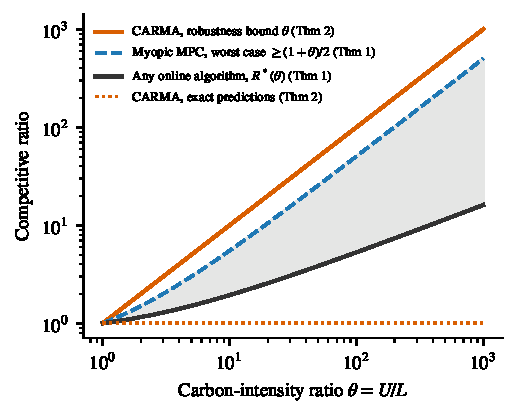
\includegraphics[width=0.62\textwidth]{../figures/fig7_ratios.pdf}
\caption{Worst-case landscape as a function of the carbon-intensity ratio $\theta$. No online algorithm can lie below $R^*(\theta)$ (Theorem~\ref{thm:lb}). Myopic MPC can be driven to $(1+\theta)/2$ even with perfect carbon forecasts. CARMA is never worse than $\theta$ (given a backstop) and is optimal when its predictions are exact (Theorem~\ref{thm:carma}).}
\label{fig:ratios}
\end{figure}

\subsection{Fair carbon attribution among sites}\label{sec:fair}

Pooling capacity reduces total emissions, but it redistributes them. Work from London is executed in South Scotland, and Scottish jobs may be displaced by it. The organisations that operate the sites (or the tenants that submit the jobs) therefore need an attribution of the pooled emissions that each of them can accept. We model this as a cooperative game. The players are the sites $\mathcal S$. A coalition $C\subseteq\mathcal S$ pools the capacity of its sites and serves the jobs submitted at them. Its stand-alone value $c(C)$ is the optimum of (\ref{eq:obj})--(\ref{eq:cap}) restricted to those jobs and sites. An attribution $\phi\in\mathbb{R}^{|\mathcal S|}$ is \emph{budget-balanced} if $\sum_o\phi_o=c(\mathcal S)$. It is in the \emph{core} if $\sum_{o\in C}\phi_o\le c(C)$ for every coalition $C$. A core attribution gives no group of sites a reason to leave the pool and schedule on its own.

Let $(\lambda,\nu,\mu)$ be optimal dual variables of the grand-coalition problem: $\lambda_j$ for the work constraint (\ref{eq:work}), $\nu_{jt}\le 0$ for the width constraint (\ref{eq:width}) and $\mu_{st}\le 0$ for the capacity constraint (\ref{eq:cap}). Define the \emph{dual carbon attribution}
\begin{equation}\label{eq:phi}
\phi_o=\sum_{j:\,o_j=o}\Big(\lambda_j w_j+\sum_t \nu_{jt}m_j\Big)+\sum_t\mu_{ot}K_o(t).
\end{equation}
Site $o$ is charged the carbon shadow price of the work it submits and is credited ($\mu\le 0$) with the shadow value of the capacity it contributes.

\begin{theorem}[Core-stable carbon attribution]\label{thm:core}
The attribution (\ref{eq:phi}) is budget-balanced and in the core of the pooling game. In particular, it is individually rational: no site is charged more than its stand-alone optimum $c(\{o\})$. It is obtained from the node potentials of the min-cost flow of Proposition~\ref{prop:flow}, at no extra computational cost.
\end{theorem}

The result follows from Owen's theorem on linear production games~\cite{owen1975core}. Games defined by network flows are known to be totally balanced~\cite{kalai1982totally}. Carbon reporting is done after the fact, so the hindsight game is the relevant object for accounting. The simpler \emph{location-based} attribution, in which each site is charged the emissions of its own jobs wherever they ran, carries no such guarantee. Section~\ref{sec:res_fair} shows that in practice it violates the core in every test week, whereas the dual attribution never does for the hindsight benchmark.

\section{Results}\label{sec:results}

\subsection{Carbon-intensity data and forecasts}\label{sec:res_forecast}

Fig.~\ref{fig:data} shows the regional intensities. Over 2022--2024, mean intensity was 37~gCO$_2$/kWh in South Scotland, 58 in North West England, 156 in the West Midlands and 163 in London. At any hour the gap between the cleanest and dirtiest site is therefore large, which is what makes spatial shifting attractive. Intensities fell steadily: London's annual mean dropped from 202~gCO$_2$/kWh in 2022 to 124 in 2024. Diurnal profiles peak in the early evening (around 18:00 UTC), and the profile of South Scotland is much flatter than those of the southern sites. The four series are positively correlated (pairwise correlations between 0.50 and 0.87), because national wind output drives all of them.

\begin{figure}[t]
\centering
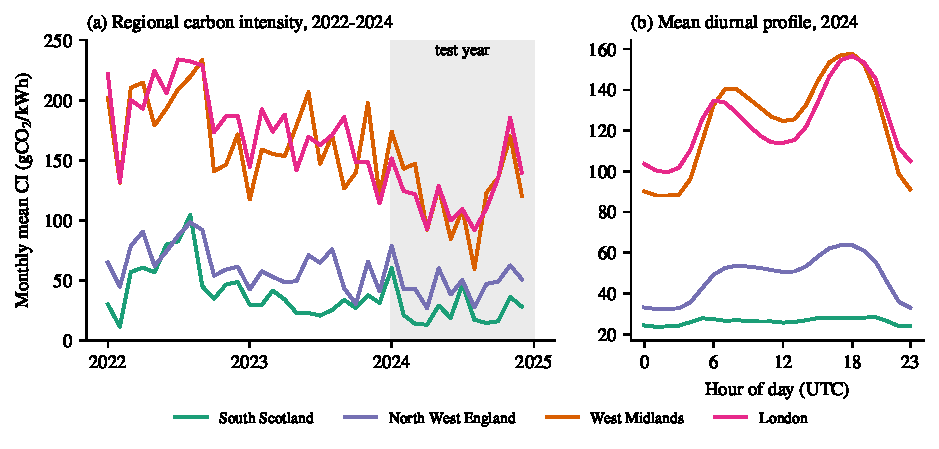
\includegraphics[width=\textwidth]{../figures/fig2_data.pdf}
\caption{Hourly carbon intensity of the four candidate sites (NESO regional data). (a) Monthly means, 2022--2024; the shaded area is the out-of-sample test year. (b) Mean diurnal profile in 2024 (UTC).}
\label{fig:data}
\end{figure}

Table~\ref{tab:forecast} and Fig.~\ref{fig:forecast}a summarise forecast accuracy in 2024. The forecaster was trained on 1.24 million (issue time, site, horizon) samples in about one minute. Averaged over horizons and sites, the direct GBM forecaster has a mean absolute error (MAE) of 31.2~gCO$_2$/kWh, against 34.4 for persistence and 40.4 for the seasonal-naive forecast. The advantage is largest at short and medium horizons: MAE falls by 23\% at 1 hour (6.2 against 8.0) and by 23\% at 6 hours (23.3 against 30.2). Beyond about 18 hours, all methods converge to the seasonal-naive level, and at 24 hours the GBM is slightly worse than the seasonal-naive benchmark. Without weather forecasts, day-ahead changes in wind output are hard to predict from the intensity history alone~\cite{maji2022carboncast}. By site, the GBM is most accurate for the volatile southern sites. In South Scotland, where intensity is low and often flat, persistence is marginally better.

\begin{table}[t]
\centering
\caption{Forecast accuracy on the 2024 test year (MAE in gCO$_2$/kWh; mean over sites unless stated).}
\label{tab:forecast}
\small
\begin{tabular}{lrrrrrrr}
\toprule
 & \multicolumn{5}{c}{Horizon $h$ (hours)} & \multicolumn{2}{c}{All horizons} \\
\cmidrule(lr){2-6}\cmidrule(lr){7-8}
Model & 1 & 3 & 6 & 12 & 24 & MAE & RMSE \\
\midrule
Persistence & 8.0 & 19.3 & 30.2 & 37.4 & 40.4 & 34.4 & 48.4 \\
Seasonal naive (24 h) & 40.4 & 40.4 & 40.4 & 40.4 & 40.4 & 40.4 & 57.0 \\
Direct GBM (this study) & \textbf{6.2} & \textbf{14.9} & \textbf{23.3} & \textbf{33.9} & 42.4 & \textbf{31.2} & \textbf{41.0} \\
\bottomrule
\end{tabular}

\smallskip
\parbox{0.92\textwidth}{\footnotesize MAE by site over all horizons (persistence / GBM): South Scotland 14.1 / 16.2; North West England 24.7 / 21.8; West Midlands 56.1 / 49.3; London 42.7 / 37.6.}
\end{table}

\begin{figure}[t]
\centering
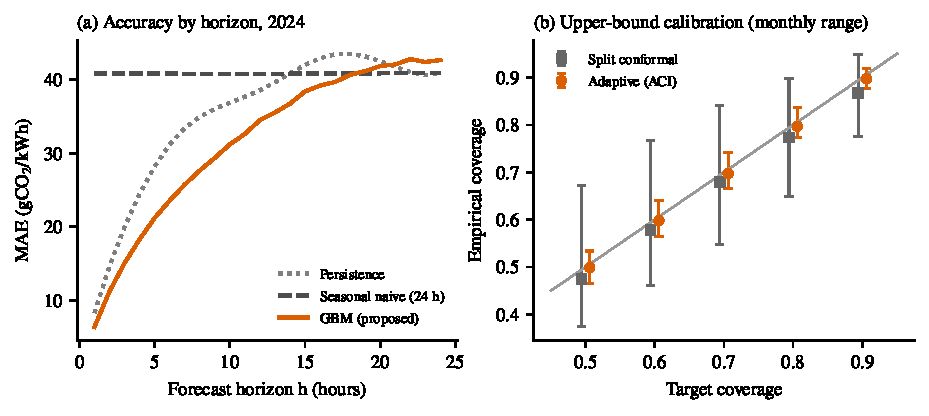
\includegraphics[width=\textwidth]{../figures/fig3_forecast.pdf}
\caption{Forecast evaluation in 2024. (a) MAE by horizon, averaged over sites. (b) Empirical coverage of one-sided upper bounds $U^\beta$ against the target level $\beta$ for static split conformal calibration and adaptive conformal inference (ACI). Markers show the annual coverage and bars the range across the 12 months.}
\label{fig:forecast}
\end{figure}

Calibration matters more than point accuracy for the risk-adjusted cost view, and Fig.~\ref{fig:forecast}b shows the effect of distribution shift. Static split-conformal bounds, calibrated on July--September 2023, under-cover in 2024 at every level: at $\beta=0.9$, annual coverage was 0.858 and monthly coverage ranged from 0.68 to 0.95. With ACI, annual coverage matches the target to within 0.002 at all levels (0.500, 0.599, 0.698, 0.798 and 0.898). Monthly coverage stays within $\pm 4$ percentage points of the target, and coverage is uniform across horizons. At $\beta=0.5$, the ACI-adjusted median lies on average 9.9~gCO$_2$/kWh below the point forecast, which reflects the downward drift in intensity that the static model does not capture.

\subsection{Hyperparameter tuning}\label{sec:tuning}

Fig.~\ref{fig:tuning} reports the validation results (13 weeks, October--December 2023, $\rho\in\{0.3,0.5,0.7\}$, migration allowed). Anticipating demand helps across the whole grid: every tested configuration beats myopic MPC, whose mean gap to the oracle is 20.3\%. The gap is smallest around $\kappa=1$, where expected demand is anticipated without inflation. For $\ell=12$ it falls to 7.3\%, and for $\ell=18$ to 7.2\%. Over-anticipation ($\kappa=1.25$ with $\ell=18$) reserves too much clean capacity and is penalised. We selected $\kappa=1$ and $\ell=12$ hours. Configurations within 0.25 percentage points of the best were resolved towards the shorter look-ahead, which keeps the network smaller.

\begin{figure}[t]
\centering
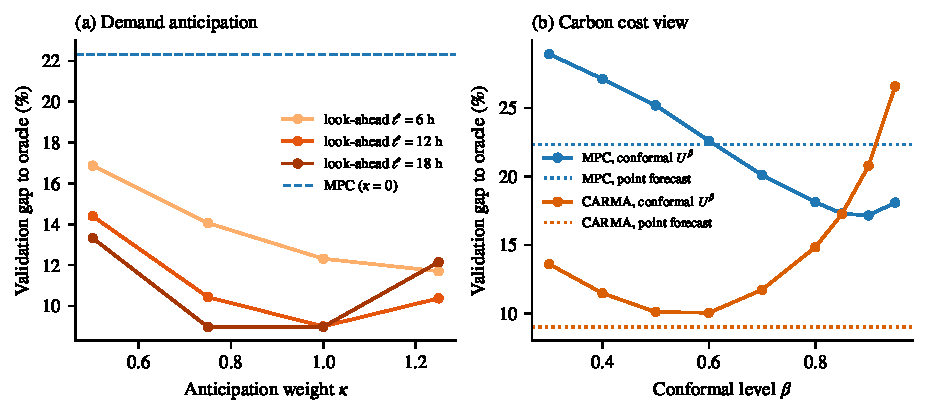
\includegraphics[width=\textwidth]{../figures/fig6_tuning.pdf}
\caption{Validation results (2023-Q4, mean over 13 weeks and three load levels). (a) Gap to the oracle as a function of the anticipation weight $\kappa$ and look-ahead $\ell$, using point forecasts. (b) Effect of the carbon cost view: conformal upper quantiles $U^\beta$ against point forecasts, for myopic MPC and for CARMA ($\kappa=1$, $\ell=12$).}
\label{fig:tuning}
\end{figure}

The cost view shows a clear interaction with anticipation (Fig.~\ref{fig:tuning}b). For myopic MPC, pessimistic conformal costs help substantially. The gap falls monotonically from 23.1\% at $\beta=0.5$ to 16.2\% at $\beta=0.8$, well below the 20.3\% obtained with point forecasts. For CARMA, every conformal level is worse than the point forecast: the best level, $\beta=0.6$, gives 8.2\% against 7.3\%. The explanation is that a risk premium on future hours makes the planner run work now rather than later, which keeps future clean capacity free. For a myopic planner this is a crude form of anticipation. Once CARMA represents future demand explicitly, the same premium double-counts it and gives up useful deferrals. The selected CARMA therefore uses point forecasts. For the test we keep MPC+conformal at $\beta=0.8$ and CARMA+conformal at $\beta=0.6$ as ablations.

\subsection{Out-of-sample scheduling performance}\label{sec:res_main}

Tables~\ref{tab:main} and~\ref{tab:main_t} report results for the 52 test weeks of 2024. Weekly traces contain on average 920, 1{,}529 and 2{,}144 jobs (69{,}900, 115{,}600 and 162{,}600 server-hours) at $\rho=0.3$, 0.5 and 0.7. Fig.~\ref{fig:gap} shows the gaps to the oracle with 95\% confidence intervals.

\begin{table}[p]
\centering
\caption{Out-of-sample results in the spatio-temporal regime (migration allowed), 52 weeks of 2024. Emis.: mean weekly operational emissions (tCO$_2$). Red.: reduction relative to ASAP-Local (\%). Gap: excess over the clairvoyant oracle (\%). Late: share of work finished after its deadline (\%). Mig.: share of work executed away from its origin (\%). $p$: Holm-adjusted two-sided Wilcoxon signed-rank test of weekly emissions against CARMA. The best gap among implementable online policies is in bold.}
\label{tab:main}
\footnotesize
\begin{tabular}{llrrrrrl}
\toprule
Load & Policy & Emis. & Red. & Gap & Late & Mig. & $p$ \\
\midrule
\inputtable{../results/table_main_st.tex}
\bottomrule
\end{tabular}
\end{table}

\begin{table}[p]
\centering
\caption{Out-of-sample results in the temporal-only regime (no migration), 52 weeks of 2024. Columns as in Table~\ref{tab:main}. Greedy-Spatial is omitted because without migration it coincides with ASAP-Local.}
\label{tab:main_t}
\footnotesize
\begin{tabular}{llrrrrl}
\toprule
Load & Policy & Emis. & Red. & Gap & Late & $p$ \\
\midrule
\inputtable{../results/table_main_t.tex}
\bottomrule
\end{tabular}
\end{table}

\begin{figure}[t]
\centering
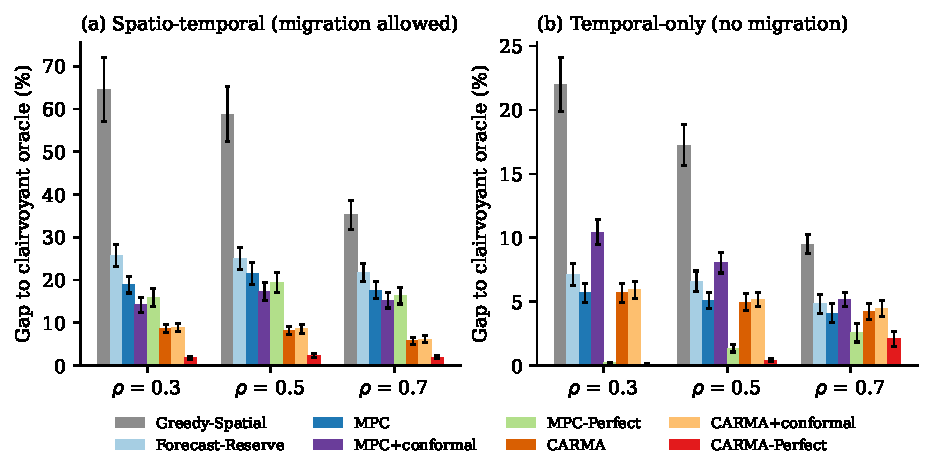
\includegraphics[width=\textwidth]{../figures/fig4_gap.pdf}
\caption{Mean gap to the clairvoyant oracle over the 52 test weeks of 2024 with 95\% confidence intervals. ASAP-Local is omitted (gap 68--275\% with migration, 9--22\% without).}
\label{fig:gap}
\end{figure}

\paragraph{Spatio-temporal regime} Carbon-aware scheduling gives large reductions when migration is allowed. The oracle cuts emissions relative to ASAP-Local by 70.5\%, 56.7\% and 39.5\% at $\rho=0.3$, 0.5 and 0.7. The achievable reduction shrinks with load because less clean capacity is left per unit of work. Greedy-Spatial realises only part of this potential (gaps of 35--65\%), because it has no temporal flexibility and floods the cleanest site with whatever arrives first. Forecast-Reserve and MPC come closer, with gaps of 18--26\%. CARMA reduces emissions by 68.1\%, 53.3\% and 36.1\% and reaches gaps of 8.7\%, 8.2\% and 5.8\%. Relative to MPC this is a further emission reduction of 7.6\%, 9.4\% and 8.8\%, and the gap to the optimum shrinks by a factor of 2.2--3.0. CARMA's emissions are lower than MPC's in 51, 52 and 52 of the 52 weeks, and lower than Forecast-Reserve's in every week (Fig.~\ref{fig:weekly}b). All differences between CARMA and the online baselines are significant after Holm correction ($p<0.001$). The only exception is CARMA+conformal at $\rho=0.3$ ($p=0.12$). CARMA also finishes more work on time under heavy load: at $\rho=0.7$, 0.05\% of its work is late, against 2.0\% for MPC, 1.2\% for Forecast-Reserve and 6.5\% for ASAP-Local. Reserving clean capacity for urgent arrivals also reserves capacity in general. CARMA migrates about the same share of work as MPC (31--70\%), so its advantage comes from better timing of the use of scarce clean capacity, not from moving more data. For a fleet of 1{,}700 batch servers at $\rho=0.5$, the difference between CARMA and MPC is 0.31~tCO$_2$ per week. The difference from carbon-agnostic operation is 3.16~tCO$_2$ per week.

\begin{figure}[t]
\centering
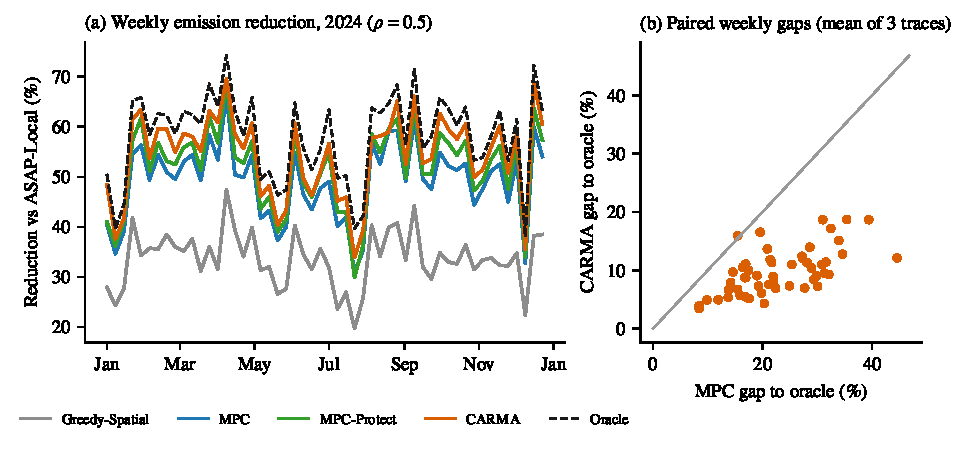
\includegraphics[width=\textwidth]{../figures/fig5_weekly.pdf}
\caption{Weekly results in 2024 (spatio-temporal regime, $\rho=0.5$). (a) Emission reduction relative to ASAP-Local. (b) Paired weekly gaps to the oracle; points below the diagonal are weeks in which CARMA outperforms MPC.}
\label{fig:weekly}
\end{figure}

\paragraph{Value of information} The clairvoyant variants separate two sources of loss. With perfect intensity forecasts, the myopic MPC-Perfect still has gaps of 15.9\%, 19.5\% and 16.3\%. Perfect carbon foresight is thus worth only 1.3--3.0 percentage points to a myopic planner. Anticipating demand is worth 10.3--13.3 points (MPC versus CARMA). With both, CARMA-Perfect comes within 1.8--2.3\% of the oracle. The two kinds of information are therefore complementary. Once demand is anticipated, forecast accuracy is worth 3.9--6.8 points (CARMA versus CARMA-Perfect), two to three times more than for the myopic planner. A myopic planner wastes clean capacity whatever its forecasts, so it cannot benefit from better ones. The weekly results in Fig.~\ref{fig:weekly}a show that the ranking is stable across seasons, although the level of achievable reductions varies from week to week with wind conditions.

\paragraph{Temporal-only regime} Without migration (Table~\ref{tab:main_t}), each job can only move in time at its origin, and the picture changes. Achievable reductions are much smaller: the oracle saves 17.7\%, 14.5\% and 8.6\%. MPC and CARMA are statistically indistinguishable here ($p\ge 0.22$), both about 4--6\% from the oracle, and both are better than Forecast-Reserve. Anticipation brings no benefit because there is no shared pool of clean capacity to protect. Each site's capacity serves only its own jobs, and the temporal windows of flexible jobs rarely collide with urgent arrivals in a way that deferral cannot absorb. In this regime the remaining loss is due almost entirely to forecast error. MPC-Perfect and CARMA-Perfect close the gap to 0.1--2.6\%, and risk-averse conformal costs make MPC worse (gaps of 5.2--10.4\%), because they suppress deferrals that would have paid off. Under heavy load ($\rho=0.7$), temporal shifting also raises lateness: the capacity at the origin sites is itself insufficient, and 6.5\% of work is late even under ASAP-Local. CARMA's late share (6.9\%) is close to that level, whereas MPC's is 13.0\%.

\paragraph{Computation} A CARMA decision takes 20--47~ms on one CPU core, against 2--7~ms for MPC. The difference comes from the ghost jobs, which enlarge the planning network. This is negligible for hourly decisions. A clairvoyant weekly oracle with up to about 2{,}700 jobs (including warm-up and trailing load) is solved exactly in under one second.

\subsection{Sensitivity analysis}\label{sec:sens}

Table~\ref{tab:sens} varies one factor at a time around the base case: spatio-temporal regime, $\rho=0.5$, $\upsilon=0.3$, $\eta=0.02$~kWh/GB. Each setting uses 26 alternating test weeks of 2024 with fresh workload seeds. CARMA keeps its hyperparameters from the base case. CARMA has the smallest gap of all online policies in every setting. Its weekly emissions are below MPC's in 155 of the 156 setting-weeks, and every comparison with a baseline is significant (all $p<10^{-7}$).

\begin{table}[t]
\centering
\caption{Sensitivity analysis (spatio-temporal regime; 26 alternating weeks of 2024 per setting; base case $\rho=0.5$, $\upsilon=0.3$, $\eta=0.02$~kWh/GB). Oracle red.: emission reduction of the oracle relative to ASAP-Local (\%). Gap columns: excess over the oracle (\%). Wins: weeks in which CARMA emits less than MPC. Late: share of late work (\%), MPC / CARMA.}
\label{tab:sens}
\footnotesize
\resizebox{\textwidth}{!}{%
\begin{tabular}{lrrrrrrr}
\toprule
 & Oracle & \multicolumn{4}{c}{Gap to oracle (\%)} & Wins vs & Late (\%) \\
\cmidrule(lr){3-6}
Setting & red. & Greedy-Sp. & F.-Reserve & MPC & CARMA & MPC & MPC / CARMA \\
\midrule
\inputtable{../results/table_sens.tex}
\bottomrule
\end{tabular}}
\end{table}

\paragraph{Share of urgent jobs} The benefit of anticipation grows with the share of urgent work, because urgent arrivals are precisely the demand that myopic planners crowd out. With $\upsilon=0.5$, CARMA's gap is 5.8\% against 20.3\% for MPC, and it has no late work (MPC 0.15\%). With $\upsilon=0.1$, the gap is 10.4\% against 20.9\%. When almost all work is flexible, there is less urgent demand to protect capacity for.

\paragraph{Network energy intensity} The ranking is unchanged over a twelve-fold range of transmission energy intensity. Cheaper transfers ($\eta=0.005$~kWh/GB) raise the oracle's reduction to 60.7\%, and CARMA's gap is 9.4\% against 25.0\% for MPC. Expensive transfers ($\eta=0.06$~kWh/GB) lower the oracle's reduction to 52.3\%, with gaps of 7.4\% and 18.1\%. The share of migrated work changes only modestly (49--51\% for CARMA), because the intensity difference between South Scotland and London is far larger than any plausible transfer overhead.

\paragraph{Misspecified demand profile} CARMA's ghost jobs come from a profile learned at $\rho=0.5$. When the actual load is 20\% higher ($\rho=0.6$), so that CARMA under-anticipates, its gap is 6.9\% against 22.1\% for MPC, and its late share is 0.01\% against 0.34\%. When the actual load is 20\% lower ($\rho=0.4$), so that it over-anticipates, CARMA reserves more clean capacity than needed. Its gap rises to 10.8\%, but that is still half of MPC's 21.3\%, and CARMA wins in 25 of the 26 weeks. Anticipation is therefore robust to moderate errors in the demand profile in both directions. The operational safeguard is the softer penalty on ghost jobs: the planner never accepts lateness of real work in exchange for serving ghost demand.


\section{Discussion}\label{sec:discussion}

\subsection{Managerial implications}

\paragraph{Protect scarce clean capacity} The largest operational loss in multi-site carbon-aware scheduling does not come from imperfect carbon forecasts. It comes from spending low-carbon capacity on work that could have waited or run elsewhere. Proposition~\ref{prop:myopic} and Theorem~\ref{thm:lb} show this in the worst case, and the 2024 experiments confirm it empirically: with migration allowed, a myopic planner with perfect foresight of carbon intensity is still 16--20\% above the optimum. For operators, clean capacity at a low-carbon site should be treated as a scarce resource with an opportunity cost, much as yield managers protect seats for high-fare late bookings. CARMA sets this protection level implicitly, through ghost jobs learned from the operator's own history, and needs no hand-tuned reservation thresholds.

\paragraph{Invest in forecasts where they pay} The value of better intensity forecasts depends on the rest of the policy. For a myopic multi-site planner, perfect forecasts are worth only 1--3 percentage points. Once demand is anticipated, they are worth 4--7 points. When work cannot migrate, they are worth almost the whole remaining gap. Forecasting effort, for example the integration of numerical weather predictions~\cite{maji2022carboncast,lowry2018day}, should therefore follow, not precede, the fix of demand myopia in multi-site settings. In single-site temporal shifting it is the main lever.

\paragraph{Use risk premia with care} Calibrated uncertainty is valuable, and ACI kept coverage on target through a year of strong decarbonisation drift. Its best use in scheduling is not obvious, however. A pessimistic carbon price improved a myopic planner by acting as a crude substitute for anticipation, but it degraded CARMA and hurt temporal-only scheduling, where it suppressed good deferrals. Because the planner re-optimises every hour, much of the protection that a risk premium would buy is already provided by recourse. Calibrated quantiles are better suited to reporting and to service-level decisions than to inflating costs by default.

\paragraph{Guarantees an operator can rely on} Worst-case properties matter for adoption, because an operator must bound the damage that a wrong forecast or an unusual week can do. Theorem~\ref{thm:carma} gives three such bounds. With a backstop resource, bad predictions can never make a job late. Emissions are never more than a factor $\theta$ above the clairvoyant optimum. Excess emissions grow at most linearly with prediction error, and the controlled-error experiments confirm this degradation profile. Theorem~\ref{thm:lb} also sets expectations: no scheduler can promise near-optimal worst-case emissions without some knowledge of future demand, so maintaining a demand profile is a necessity, not a refinement.

\paragraph{Fair carbon accounting for shared capacity} Pooling halved the emissions of the four sites, but location-based accounting, which charges each site for its own jobs wherever they run, would have made South Scotland and North West England worse off than on their own in almost every week. A multi-organisation or multi-tenant pool attributed this way is unstable, because its cleanest members have an incentive to leave. The dual attribution of Theorem~\ref{thm:core} charges each site the carbon shadow price of its demand and credits it for the capacity it contributes. It is budget-balanced, no coalition would prefer to secede, and it is a by-product of the scheduling problem. It offers a principled basis for internal carbon pricing, for sharing the benefits of carbon-aware scheduling among business units, and for tenant-level carbon reporting in shared data centres.

\paragraph{Deployment} CARMA needs three inputs: a public carbon-intensity feed, a demand profile computed from the operator's own job logs, and a network-flow solver. It decides within tens of milliseconds and returns a plan that is optimal for its model, which makes its decisions auditable. This supports the transparency expected of carbon claims in sustainability reporting. The algorithm is also a rare case in which lower emissions come with better service: under heavy load, CARMA finished far more work on time than the other forecast-driven planners (0.05\% late work, against 1.2--2.0\%).

\subsection{Limitations and future research}

The study has several limitations. First, workloads are synthetic. The generator has realistic features (diurnal and weekly seasonality, heavy-tailed job sizes, a mix of urgent and flexible jobs, width limits), but results on production traces may differ. In particular, CARMA's advantage depends on how predictable arrivals are, and the sensitivity analysis shows how it degrades when the load deviates from the learned profile. Second, we use average (attributional) regional intensities as published by NESO. Marginal emission factors may be more appropriate for evaluating load shifting~\cite{dodge2022measuring}, and regional values in Great Britain are modelled estimates, not metered data. Third, the facility parameters (PUE, network energy) are stylised, idle server power is not modelled, and embodied emissions are outside the scope of this study~\cite{acun2023carbon}. Fourth, the forecaster deliberately excludes weather forecasts, so its day-ahead skill is limited. Fifth, bag-of-tasks jobs with free preemption and migration are an idealisation. Jobs with state, data-gravity or data-sovereignty constraints would add restrictions that break the pure network structure. Sixth, the guarantees of Theorem~\ref{thm:carma} assume a backstop resource and a positive emission floor, and the smoothness bound assumes that the planning window covers the episode. The simulations use neither a backstop nor episodes that short, so they test the predicted behaviour rather than the bound itself. The core property of Theorem~\ref{thm:core} is exact for the hindsight benchmark; for CARMA's realised emissions it held in all but 5 of 728 coalition checks.

Several extensions follow naturally. The ghost-demand profile could be replaced by probabilistic arrival forecasts, with the anticipation weight set by a newsvendor-type argument. Scenario-based or distributionally robust variants could treat demand and carbon uncertainty jointly~\cite{bertsimas2004price}. The framework can also be coupled with on-site renewables and storage~\cite{souza2023ecovisor,acun2023carbon} and with demand-response programmes~\cite{wierman2014opportunities}. Finally, the robustness guarantee could be tightened from $\theta$ towards the $\Theta(\sqrt\theta)$ lower bound, for example by protecting deferral decisions with reservation prices~\cite{elyaniv2001optimal,lechowicz2025learning} while retaining consistency, and the attribution could be extended to online, per-decision carbon prices.

\section{Conclusions}\label{sec:conclusion}

This paper studied carbon-aware scheduling of deferrable computing workloads across data-centre sites as a sustainable-operations problem. We showed that the offline problem, including width limits, deadlines and the emissions of data transfer, is a minimum-cost flow. This yields exact oracles and fast online planning. We proved that uncertainty about demand alone forces every online algorithm to a competitive ratio of order $\sqrt\theta$, even with perfect carbon forecasts, and that myopic planning does far worse. We proposed CARMA, which augments the planning network with ghost jobs for expected arrivals, and a probabilistic carbon-intensity forecaster with adaptive conformal calibration. We proved that CARMA meets every deadline and is $\theta$-competitive under any predictions, optimal under exact predictions and smooth in between. The dual prices of the pooled problem also yield a carbon attribution that is in the core of the pooling game. In 52 out-of-sample weeks of 2024 on British regional grid data, CARMA cut emissions relative to carbon-agnostic operation by 36--68\% when migration was allowed. That is within 6--9\% of the clairvoyant optimum and 7.6--9.4\% below myopic MPC, and CARMA also reduced late work. Anticipating demand was worth far more than perfect carbon foresight, while risk-averse carbon pricing helped only myopic planners. CARMA degraded gracefully under injected prediction errors. Location-based carbon accounting violated coalitional stability in every test week. The dual attribution never did for the hindsight benchmark, and failed only 5 of 728 checks for CARMA's realised emissions. When jobs cannot migrate, achievable reductions are smaller (9--18\%) and forecast accuracy is the binding constraint. Carbon-aware computing is most effective when schedulers plan for the work that has not yet arrived, not only for the grid conditions that lie ahead.


\section*{CRediT authorship contribution statement}
\textbf{Quang-Vinh Dang:} Conceptualization, Methodology, Software, Data curation, Formal analysis, Investigation, Validation, Visualization, Writing -- original draft, Writing -- review \& editing.

\section*{Declaration of competing interest}
The author declares no known competing financial interests or personal relationships that could have appeared to influence the work reported in this paper.

\section*{Funding}
This research did not receive any specific grant from funding agencies in the public, commercial, or not-for-profit sectors.

\section*{Data availability}
The carbon-intensity data are publicly available from the NESO Carbon Intensity API~\cite{nesoapi} under the CC BY 4.0 licence. The generation-mix data of the additional grids are publicly available from Energy-Charts, the EIA-930 bulk files, the ONS open-data portal and the New Zealand Electricity Authority. The data snapshot used in this study, all code, the workload generator with fixed random seeds, and all raw experiment outputs are available from the author's repository (\url{https://github.com/vinhqdang/Sustainable-Operations-and-Computers}).

\appendix
\setcounter{figure}{0}\setcounter{table}{0}
\makeatletter\@addtoreset{figure}{section}\@addtoreset{table}{section}\makeatother
\renewcommand{\thefigure}{\Alph{section}.\arabic{figure}}
\renewcommand{\thetable}{\Alph{section}.\arabic{table}}
\section{Proofs}\label{app:proofs}

\paragraph{Atoms} Splitting a job $j$ into sub-jobs $j_1,\dots,j_k$ with work $w_{j_i}$ and widths $m_{j_i}=m_jw_{j_i}/w_j$ does not change the optimal value of any planning problem. Given a solution for the merged job, the allocation $x_{j_i s}(t)=x_{js}(t)\,w_{j_i}/w_j$ satisfies every constraint of the split problem at the same cost. Conversely, summing the sub-job allocations gives a feasible allocation for the merged job, because $\sum_i m_{j_i}=m_j$. Splitting also preserves window-feasibility, since $w_{j_i}/m_{j_i}=w_j/m_j$. We may therefore compare true and predicted job sets atom by atom.

\subsection{Proof of Theorem~\ref{thm:lb}}

Normalise $L=1$, so $U=\theta$. Site $A$ has one server with cost $p\in[1,\theta]$ in hour 0 and cost 1 in hour 1. Site $B$ has ample capacity at cost $\theta$ in both hours. Transfer costs are zero. A flexible job ($w=m=1$, window $\{0,1\}$) is released at $t=0$. The adversary either releases nothing more (scenario 1) or releases an urgent job ($w=m=1$, window $\{1\}$) at $t=1$ (scenario 2). All costs are known in advance.

Consider any deterministic online algorithm that may split work fractionally, and let $x\in[0,1]$ be the amount of flexible work it runs at $t=0$. Running at $B$ in hour 0 costs $\theta\ge p$ and is dominated, so we may assume this work runs at $A$. In scenario 1 the algorithm finishes the remaining $1-x$ at $A$ in hour 1, so $\mathrm{ALG}_1=xp+(1-x)$, while $\mathrm{OPT}_1=1$. In scenario 2, hour 1 must process $2-x$ units and $A$ can take only one of them, so $\mathrm{ALG}_2=xp+1+(1-x)\theta$, while $\mathrm{OPT}_2=p+1$. The ratio $r_1(x)=1+x(p-1)$ increases in $x$, and the ratio $r_2(x)=\big(1+\theta-x(\theta-p)\big)/(p+1)$ decreases in $x$. Hence $\min_x\max\{r_1,r_2\}$ is attained where they are equal, at $x^*=(\theta-p)/(p^2-p-1+\theta)\in[0,1]$, and its value is
\[
1+\frac{(p-1)(\theta-p)}{p^2-p-1+\theta}.
\]
The adversary chooses $p$ to maximise this value, which gives $R^*(\theta)$. The choice $p=\sqrt\theta$ gives the stated closed-form lower bound. For a randomised algorithm, the expected cost in each scenario is affine in $x$, so it equals the cost of the deterministic fractional algorithm that plays $\mathbb{E}[x]$, and the bound applies against an oblivious adversary. Myopic MPC sees only the flexible job at $t=0$ and defers it entirely to the cheaper hour 1 ($x=0$). With $p\to 1^+$, its ratio in scenario 2 tends to $(1+\theta)/2$. \hfill$\square$

\subsection{Proof of Theorem~\ref{thm:carma}}

\paragraph{Robustness} We first show by induction that every pending real job $j$ is window-feasible at the start of every hour: its remaining work satisfies $r_j\le m_j(d_j-t)$. This holds at release by (A1). Suppose it holds at hour $t$, and suppose the plan of CARMA leaves some real work $u_j>0$ unfinished. Because $r_j\le m_j(d_j-t)$, some hour $\tau\in[t,d_j)$ carries less than $m_j$ units of job $j$ in the plan. Moving a small amount of $u_j$ to the backstop in hour $\tau$ keeps the plan feasible, because the backstop has unlimited capacity, and it changes the cost by a negative amount, because the backstop costs at most $U<\Pi$. This contradicts optimality, so the plan completes all real work. After the first hour is executed, the rest of the plan is a feasible completion, so $r_j'\le m_j(d_j-t-1)$ and the induction step holds. No real job is ever late. Every executed server-hour costs at most $U$, so $\mathrm{ALG}\le U\,W$, where $W$ is the total work. Every server-hour in the oracle's solution costs at least $L$, and slack costs $\Pi>U\ge L$, so $\mathrm{OPT}\ge LW$. Hence $\mathrm{ALG}\le\theta\,\mathrm{OPT}$.

\paragraph{Telescoping} Let $\sigma_t$ be the state at the start of hour $t$: the remaining work of all real jobs released by $t$. Let $V_t(\sigma,G;c)$ be the optimal value of (\ref{eq:obj})--(\ref{eq:cap}) over hours $t,\dots,T-1$ for the pending jobs $\sigma$ and the future jobs $G$ under costs $c$. Write $\bar V_t=V_t(\sigma_t,F_t;c)$, so that $\bar V_0=\mathrm{OPT}$ and $\bar V_T=0$. For a feasible hour-$t$ allocation $x$ with cost $g_t(x)$ and successor state $\sigma^+(x)$, define
\[
Q_t(x)=g_t(x)+V_{t+1}\big(\sigma^+(x),F_t;c\big),\qquad \hat Q_t(x)=g_t(x)+V_{t+1}\big(\sigma^+(x),\hat F_t;\hat c_t\big).
\]
By dynamic programming over a deterministic future, $\min_xQ_t(x)=\bar V_t$, and $Q_t(x_t)=g_t(x_t)+\bar V_{t+1}$ for the executed action $x_t$. Summing over $t$ gives
\[
\mathrm{ALG}-\mathrm{OPT}=\sum_{t=0}^{T-1}\delta_t,\qquad \delta_t=Q_t(x_t)-\min_xQ_t(x)\ge 0.
\]
Ghost jobs are released at $t+1$ or later, the planning window reaches $T$ by (A2), and hour-$t$ costs are observed. The planning problem solved by CARMA at hour $t$ is therefore exactly $\min_x\hat Q_t(x)$, and $x_t$ is a minimiser.

\paragraph{One-step loss} Let $x^*\in\arg\min Q_t$. Since $\hat Q_t(x_t)\le\hat Q_t(x^*)$, we have $\delta_t\le\Delta(x_t)-\Delta(x^*)$, where $\Delta=Q_t-\hat Q_t$. Write $\Delta=D_1+D_2$ with
\begin{align*}
D_1(x)&=V_{t+1}(\sigma^+(x),F_t;c)-V_{t+1}(\sigma^+(x),\hat F_t;c),\\
D_2(x)&=V_{t+1}(\sigma^+(x),\hat F_t;c)-V_{t+1}(\sigma^+(x),\hat F_t;\hat c_t).
\end{align*}
\emph{Cost error.} An optimal solution under $\hat c_t$ is feasible under $c$, and its cost changes by at most $\varepsilon_t$ per unit of flow on future-hour arcs. The same holds with the roles of $c$ and $\hat c_t$ exchanged. Hence $|D_2(x)|\le\varepsilon_tW_t$ for all $x$, and $D_2(x_t)-D_2(x^*)\le 2\varepsilon_tW_t$.

\emph{Demand error.} Under (A1), the penalty attached to a window-feasible job does not affect any optimal value, provided it is at least $U$. If a solution leaves slack on such a job, the argument used for robustness moves that slack to the backstop at no greater cost. True future jobs (penalty $\Pi$) and ghost jobs (penalty $\Pi_g$) can therefore be treated as identical atoms whenever they coincide. Let $a$ be a window-feasible atom and $G$ any set of future jobs. For every state $\sigma$,
\[
Lw_a\;\le\;V(\sigma,G\cup\{a\})-V(\sigma,G)\;\le\;Uw_a.
\]
For the upper bound, add $a$ to an optimal solution for $G$ by running it on the backstop at rate $w_a/(d_a-a_a)\le m_a$ in every hour of its window. For the lower bound, delete $a$'s flow and slack from an optimal solution for $G\cup\{a\}$; each deleted unit cost at least $\min\{L,\Pi_a\}=L$, since $\Pi_a\ge U\ge L$. Now transform $\hat F_t$ into $F_t$ by removing $\hat F_t\setminus F_t$ and adding $F_t\setminus\hat F_t$, one atom at a time. Then $D_1(x)$ is a sum of increments, each lying in $[Lw_a,Uw_a]$ (with a minus sign for removals) for every $x$. Therefore $D_1(x_t)-D_1(x^*)\le(U-L)\sum_aw_a=(U-L)\,d_t$.

Combining the two bounds gives $\delta_t\le(U-L)d_t+2\varepsilon_tW_t$. Summing over $t$ and taking the minimum with the robustness bound proves (\ref{eq:smooth}). If $d_t=\varepsilon_t=0$ for all $t$, then $\delta_t=0$ and $\mathrm{ALG}=\mathrm{OPT}$. \hfill$\square$

\subsection{Proof of Theorem~\ref{thm:core}}

Write the problem of coalition $C$ as $c(C)=\min\{c^\top z: A_{=}z=b_{=}(C),\ A_{\le}z\le b_{\le}(C),\ z\ge 0\}$, where $z=(x,u)$. Jobs submitted outside $C$ have zero work and zero width, and sites outside $C$ have zero capacity. This forces the corresponding flows to zero, so the problem coincides with the stand-alone problem of $C$. The right-hand side is additive over sites: $b(C)=\sum_{o\in C}b^o$, where $b^o$ collects the work and widths of the jobs submitted at $o$ and the capacity of site $o$. The matrix $A$ and the cost $c$ do not depend on $C$. The dual problem $\max\{b(C)^\top y: A^\top y\le c,\ y_{\le}\le 0\}$ therefore has a feasible set that is the same for all coalitions.

Let $y^*=(\lambda,\nu,\mu)$ be an optimal dual solution for $\mathcal S$. The slack variables make every primal problem feasible, and costs are non-negative, so strong duality gives $c(\mathcal S)=b(\mathcal S)^\top y^*=\sum_o(b^o)^\top y^*=\sum_o\phi_o$, which is budget balance. For any coalition $C$, $y^*$ is dual-feasible for $C$, so weak duality gives $c(C)\ge b(C)^\top y^*=\sum_{o\in C}\phi_o$, which is the core condition~\cite{owen1975core}. Expanding $(b^o)^\top y^*$ gives (\ref{eq:phi}). By Proposition~\ref{prop:flow} the problem is a min-cost flow. Its optimal node potentials, together with the reduced costs they induce on saturated capacity arcs, give an optimal dual solution, so network simplex returns $y^*$ together with the optimal flow. \hfill$\square$

\section{Forecast evaluation}\label{app:forecast}

Table~\ref{tab:forecast} and Fig.~\ref{fig:forecast}a summarise forecast accuracy in 2024. Averaged over horizons and sites, the direct GBM forecaster has a mean absolute error (MAE) of 31.2~gCO$_2$/kWh, against 34.4 for persistence and 40.4 for the seasonal-naive forecast. The advantage is largest at short and medium horizons: MAE falls by 23\% at 1 hour (6.2 against 8.0) and by 23\% at 6 hours (23.3 against 30.2). Beyond about 18 hours, all methods converge to the seasonal-naive level, and at 24 hours the GBM is slightly worse than the seasonal-naive benchmark. Without weather forecasts, day-ahead changes in wind output are hard to predict from the intensity history alone~\cite{maji2022carboncast}. By site, the GBM is most accurate for the volatile southern sites. In South Scotland, where intensity is low and often flat, persistence is marginally better. Diebold--Mariano tests~\cite{diebold1995comparing} with absolute-error loss and HAC variance confirm these patterns. For the three English sites, the GBM is significantly more accurate than persistence at horizons of 1--18 hours ($p\le0.001$) and indistinguishable at 24 hours ($p\ge0.13$). For South Scotland it is significantly better at 1 hour, indistinguishable at 3 hours and significantly worse from 6 hours onwards.

\begin{table}[t]
\centering
\caption{Forecast accuracy on the 2024 test year (MAE in gCO$_2$/kWh; mean over sites unless stated).}
\label{tab:forecast}
\small
\begin{tabular}{lrrrrrrr}
\toprule
 & \multicolumn{5}{c}{Horizon $h$ (hours)} & \multicolumn{2}{c}{All horizons} \\
\cmidrule(lr){2-6}\cmidrule(lr){7-8}
Model & 1 & 3 & 6 & 12 & 24 & MAE & RMSE \\
\midrule
Persistence & 8.0 & 19.3 & 30.2 & 37.4 & 40.4 & 34.4 & 48.4 \\
Seasonal naive (24 h) & 40.4 & 40.4 & 40.4 & 40.4 & 40.4 & 40.4 & 57.0 \\
Direct GBM (this study) & \textbf{6.2} & \textbf{14.9} & \textbf{23.3} & \textbf{33.9} & 42.4 & \textbf{31.2} & \textbf{41.0} \\
\bottomrule
\end{tabular}

\smallskip
\parbox{0.92\textwidth}{\footnotesize MAE by site over all horizons (persistence / GBM): South Scotland 14.1 / 16.2; North West England 24.7 / 21.8; West Midlands 56.1 / 49.3; London 42.7 / 37.6.}
\end{table}

\begin{figure}[t]
\centering
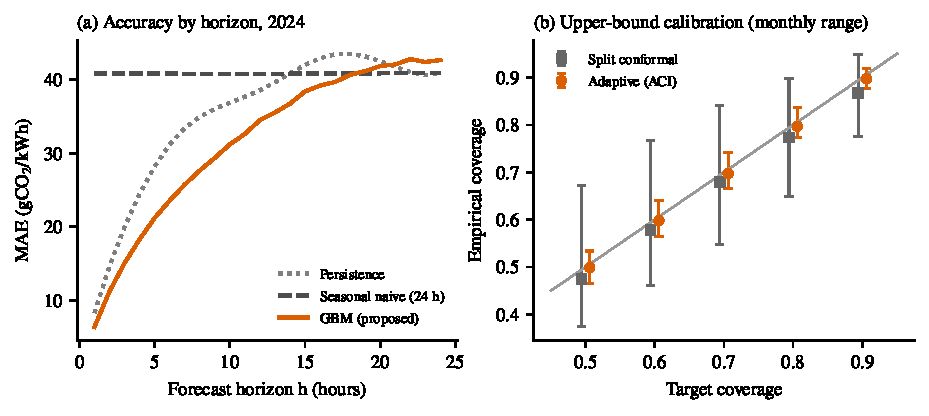
\includegraphics[width=\textwidth]{../figures/fig3_forecast.pdf}
\caption{Forecast evaluation in 2024. (a) MAE by horizon, averaged over sites. (b) Empirical coverage of one-sided upper bounds $U^\beta$ against the target level $\beta$ for static split conformal calibration and adaptive conformal inference (ACI). Markers show the annual coverage and bars the range across the 12 months.}
\label{fig:forecast}
\end{figure}

Calibration matters more than point accuracy for the risk-adjusted cost view, and Fig.~\ref{fig:forecast}b shows the effect of distribution shift. Static split-conformal bounds, calibrated on July--September 2023, under-cover in 2024 at every level: at $\beta=0.9$, annual coverage was 0.858 and monthly coverage ranged from 0.68 to 0.95. With ACI, annual coverage matches the target to within 0.002 at all levels (0.500, 0.599, 0.698, 0.798 and 0.898). Monthly coverage stays within $\pm 4$ percentage points of the target, and coverage is uniform across horizons. At $\beta=0.5$, the ACI-adjusted median lies on average 9.9~gCO$_2$/kWh below the point forecast, which reflects the downward drift in intensity that the static model does not capture. Coverage is not the whole story. In pinball loss, ACI improves on static calibration at levels 0.5--0.7 (for example 14.83 against 14.90 at 0.5) but is worse at 0.8 and 0.9 (9.06 against 8.35 at 0.9). The online recalibration buys coverage at high levels with wider bounds. Two implementation details qualify the ACI results. Feedback is delayed: the miscoverage level for horizon $h$ is updated only when the outcome is observed, $h$ hours after issue, so the adaptation lags by up to a day at long horizons. The adapted level is also clipped to $[0,1]$ and read from a quantile grid of step 0.001, so the finite-sample guarantee of ACI~\cite{gibbs2021adaptive} holds only approximately.


\section{Numerical check of Theorem~\ref{thm:carma}}\label{app:thm2check}

The weekly experiments of Section~\ref{sec:results} violate the assumptions of Theorem~\ref{thm:carma}, so we check the theorem separately in episodes that satisfy them (script \texttt{verify\_theorem2.py}). Each episode is one day ($T=24=H$ hours) of the synthetic workload, with days starting at 26 test weeks, a backstop of unlimited capacity at the episode's largest unit cost $U$ (A1), window-feasible jobs, real-job penalty $\Pi=10^4>U$ and ghost penalty $\Pi_g=U$. Ghost jobs are the true future jobs, each omitted from the predictions with probability $q$ (demand error), and the carbon forecasts of future hours receive i.i.d.\ Gaussian noise of standard deviation $\sigma$~gCO$_2$/kWh (carbon error). For each episode, we compute the clairvoyant optimum OPT with the backstop, the emissions of CARMA, and the right-hand side of the smoothness bound (\ref{eq:smooth}) from the realised $d_t$, $\varepsilon_t$ and $W_t$. There are 26 episodes for each of 12 settings (two loads and six error settings).

\begin{table}[!htbp]
\centering
\caption{Numerical check of Theorem~\ref{thm:carma} in one-day episodes with a backstop. ALG/OPT: emissions of CARMA relative to the clairvoyant optimum (mean and maximum over 26 episodes). Bound: mean ratio of the right-hand side of (\ref{eq:smooth}) to OPT. The bound held in every episode, and no real work was late.}
\label{tab:thm2}
\small
\begin{tabular}{rrrrrr}
\toprule
Load $\rho$ & $q$ & $\sigma$ & Mean ALG/OPT & Max ALG/OPT & Bound / OPT \\
\midrule
0.5 & 0 & 0 & 1.000 & 1.000 & 1.0 \\
0.5 & 0 & 25 & 1.011 & 1.031 & 37.7 \\
0.5 & 0 & 100 & 1.061 & 1.257 & 139.6 \\
0.5 & 0.1 & 0 & 1.009 & 1.072 & 6.4 \\
0.5 & 0.3 & 0 & 1.066 & 1.365 & 17.9 \\
0.5 & 0.3 & 100 & 1.094 & 1.332 & 160.2 \\
0.9 & 0 & 0 & 1.000 & 1.000 & 1.0 \\
0.9 & 0 & 25 & 1.001 & 1.003 & 19.3 \\
0.9 & 0 & 100 & 1.004 & 1.015 & 69.3 \\
0.9 & 0.1 & 0 & 1.001 & 1.011 & 3.6 \\
0.9 & 0.3 & 0 & 1.010 & 1.112 & 9.1 \\
0.9 & 0.3 & 100 & 1.010 & 1.029 & 78.2 \\
\bottomrule
\end{tabular}
\end{table}

Three observations follow. With exact predictions, CARMA reproduces the optimum to within the 0.01 server-hour quantisation of the flow solver (relative difference at most $2\times10^{-5}$), which is consistency. No real work was late in any of the 312 episodes, in line with deadline safety. The smoothness bound holds in every episode but is loose by one to two orders of magnitude when predictions are wrong, because each misprediction enters $d_t$ in every hour in which it is visible. The realised excess over the optimum is at most 37\%, so the bound is a qualitative statement that errors enter linearly, not a tight prediction.

\section{Results on other grids at all loads}\label{app:multigrid}

\begin{table}[!htbp]
\centering
\caption{Results on five grids at all loads (migration allowed; 52 test weeks of 2024). Gaps to the oracle (\%). Advantage: gap of the best baseline without demand information minus CARMA's gap, with a 95\% block-bootstrap CI (points). Late: CARMA's share of late work (\%).}
\label{tab:multigrid_loads}
\scriptsize\setlength{\tabcolsep}{2.5pt}
\begin{tabular}{lrrrrrrlrr}
\toprule
Fleet & $\rho$ & \makecell{Oracle\\red.} & MPC & \makecell{MPC-\\Prot.} & \makecell{MPC+\\conf.} & CARMA & \makecell{Best baseline} & \makecell{Advantage (CI)} & Late \\
\midrule
\inputtable{../results/table_multigrid_loads.tex}
\bottomrule
\end{tabular}
\end{table}


\bibliographystyle{elsarticle-num}
\bibliography{references}

\end{document}
